We use the \texttt{Linux kernel 3.5.0} for implementation of application domain and driver domain. We used Arch Linux on \texttt{x86\_64} platform for the IDDR system testing and performance evaluation. The specifications of the system used for the evaluation is presented in the table~\ref{tab:config}. 

\begin{table}
\caption{Hardware specifications of the system}
\begin{center}
\begin{tabular}{ll}
  \hline
  \label{tab:config}
  System Parameter & Configuration \\
  \hline
  Processor & 1 X Quad-code AMD Opteron(tm) Processor 2380, 2.49 Ghz \\
  Number of cores & 4 per processor \\
  Hyperthreading & OFF \\
  %Turbo boost & ?? \\
  L1 L2 cache & 64K/512K per core \\
  L3 cache & 6144K \\
  Main memory & 16Gb \\
  Storage & SATA, HDD 7200RPM \\
  \hline 
\end{tabular}
\end{center}
\end{table}

\section{Goals}
\label{sec:goals}
The goals of the IDDR system evaluation are:
\begin{enumerate}
\item \textbf{Comparison  of Xen's isolated driver domain with the base IDDR system:}
\\[3mm]
The goal of this thesis is to explore the performance improvement opportunity in the Xen's isolated driver domain and implement it. However, the source code for the isolated driver domain is not available in the open source Xen hypervisor. As a result, we re-implemented the isolated driver domain. We refer to the re-implementation as the base Isolated Device Driver (IDDR) system. We implemented the spinlock based communication channel over the base IDDR system. We call it as the new IDDR system.
\\[3mm]
In order to prove the performance improvement of the new IDDR system over the base IDDR system and the Xen's isolated driver domain, it is necessary to compare the performance of the Xen's isolated driver domain with the base IDDR system. The Xen's isolated driver domain follows split device driver architecture. Since the split device driver architecture has gone over decade for the performance testing, the performance Comparison with it would prove the solid baseline code of the IDDR system. 
\\[3mm]
We achieve this evaluation goal by comparing the performance of the base IDDR system with the Xen split device driver. The Comparison  shows that the performance of the IDDR system matches the performance of the Xen's isolated driver domain. Hence, proves that our implementation provides a suitable baseline for the performance improvement.

\item \textbf{An evaluation of performance improvement:}
\\[3mm] 
The second goal of the evaluation is to prove that the spinlock based communication channel improves the performance of the inter-domain communication and hence the IDDR system.
\\[3mm]
We achieve this evaluation goal by comparing the performance of the base IDDR system with the new IDDR system. The Comparison  shows that the new IDDR system performs better than the base IDDR system and the Xen's isolated driver domain.
\end{enumerate}

\section{Methodology}
\label{sec:methodology}
In order to measure the performance of the system, we run performance tests against the variety of block devices. In a Linux system, a loop device is a device that makes a file accessible as a block device. A ramdisk is a block of a memory, which acts as a disk drive. In order to cover a variety of the devices we use block devices such as SATA disk, ramdisk and loop device for the performance testing.
\\[3mm]
In order to conduct the performance tests, we format the block device with the ext2 file system, and run the fileIO SysBench benchmark~\cite{sysbench} on it. SysBench is a multi-threaded benchmark tool for evaluating a system. It evaluates the system performance without installing a database or without setting up complex database benchmarks. SysBench benchmark has different test modes. FileIO is one of the test mode which can be used to produce various file I/O workloads. It can run a specified number of threads by executing all requests in parallel. We run SysBench benchmark in a fileIO test mode to generate 128 files with \texttt{1Gb} of total data. We execute random reads, random writes, mix of random read-writes, sequential reads, sequential writes and mix of sequential reads and writes on all the three devices. The block size is kept as \texttt{16Kb}. We vary the number of SysBench threads from 1 to 32, to get the throughput of the system under different workload. 

\section{Xen Split Device Driver vs Base IDDR System}
As per our first goal of evaluation mentioned in Section~\ref{sec:goals}, we compare the base IDDR with the Xen split device driver. 

\subsection*{Experimental Setup}

\subsubsection*{Xen Split Device Driver}
We create a ramdisk in the domain 0. The guest domain (domain U) is configured such that the ramdisk uses a split device driver and is available in the guest domain. We do a similar setup for the loop device and the SATA disk. In case of loop device, we create a loop device in the domain 0 and then configure the guest domain to use the loop device as a disk. In case of SATA disk, we configure the guest domain to use SATA disk as a secondary disk. We format and mount the disk in the guest domain with the ext2 file system. SysBench benchmark is run on the mounted partition as explained in section~\ref{sec:methodology}.

\subsubsection*{Base IDDR System}
In a Xen hypervisor, the domain 0 always runs as a paravirtualized guest and in our setup we run the domain U as a HVM guest.
\\[3mm] 
In Xen, paravirtualized guest is a guest which is aware of the VMM and require special ported kernel to run efficiently without emulation or virtual emulated hardware. Paravirtualization does not require virtualization extensions from the host CPU. 
\\[3mm]
On the other hand, fully virtualized or hardware virtual machine (HVM) guest require CPU virtualization extensions such as Intel VT, AMD-V. The Xen uses modified version of Qemu to emulate hardware for HVM guests. CPU virtualization extensions help to boost the performance of the emulation. A fully virtualized guest does not require special kernel. In order to boost the performance, fully virtualized HVM guest uses special paravirtual device drivers and bypasses the emulation for disk and network IO.
\\[3mm]
A HVM guest is expected to have less syscall overhead and faster memory bandwidth than a PV guest. In the Xen split device driver setup, the backend device driver runs in the domain 0 and the frontend device driver runs in a domain U. In order to compare the Xen split device driver and the base IDDR system, it is necessary to have the setup similar to the Xen split device driver. We run the backend driver in the domain 0 and the frontend driver in the domain U.
\\[3mm]
We insert a ramdisk and the base IDDR system's backend module in the domain 0 and the frontend module in the guest domain (domain U). We format and mount the ramdisk with ext2 file system and run the SysBench benchmark on it.  
\\[3mm]
Similar setup is used for a loop device. We create a loop device in the domain 0 and insert the backend driver in the same domain. We insert the frontend module in the guest domain.

\subsubsection*{Comparison }
We compare the throughput of the Xen split device driver and the base IDDR system in Figure~\ref{fig:iddrvsxen-ramdisk-rdwr} and Figure~\ref{fig:iddrvsxen-loop-rd}. The Figure~\ref{fig:iddrvsxen-ramdisk-rdwr} presents throughput of both systems when data is randomly read from a ramdisk and at the same time written to it. Figure~\ref{fig:iddrvsxen-loop-rd} presents throughput when data is randomly read from a loop device. 
\\[3mm]
On a loop device, the performance of the base IDDR system differs by 3\%-4\% when compared to xen split device driver. On a ramdisk, the throughput of the base IDDR system matches that of the Xen split device driver. This proves that our implementation of the isolated driver domain provides a suitable baseline for the performance improvement.

\begin{figure}[!ht]
%\centering
  \begin{subfigure}[b]{0.2\textwidth}
  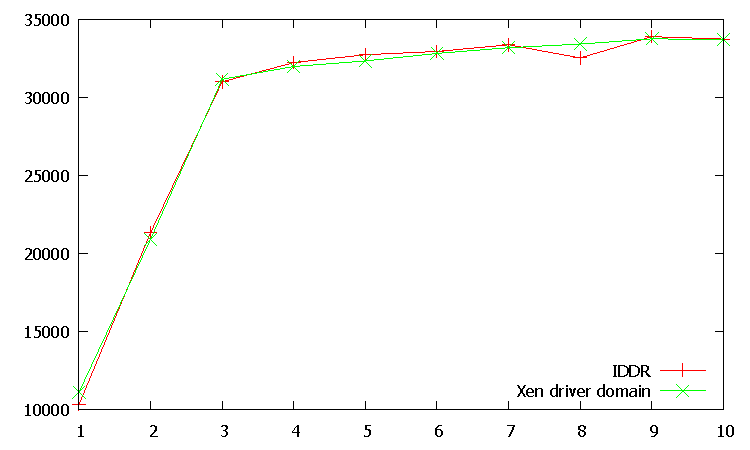
\includegraphics[scale=.7]{iddrvsxen-ramdisk-rdwr}
  \caption{Random reads-writes on a ramdisk}
  \label{fig:iddrvsxen-ramdisk-rdwr}
  \end{subfigure}
  \hspace{50mm}
  %\hfill
  \begin{subfigure}[b]{0.2\textwidth}
  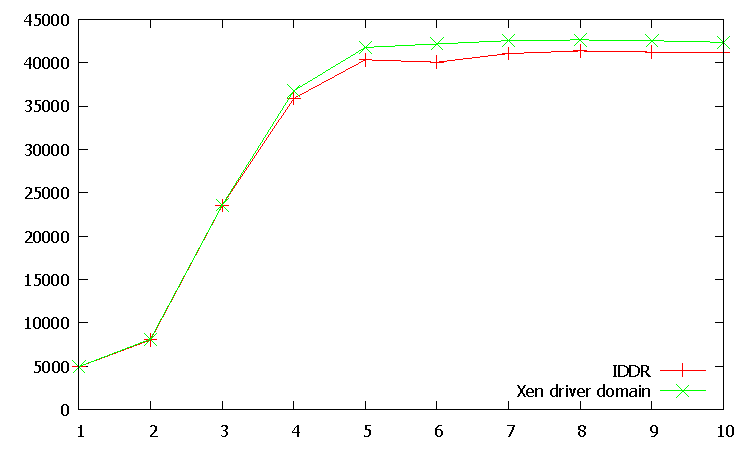
\includegraphics[scale=.7]{iddrvsxen-loop-rd}
  \caption{Random reads on a loop device}
  \label{fig:iddrvsxen-loop-rd}
  \end{subfigure}\\
\caption{Base IDDR system vs Xen split driver}\label{fig:seqloopdisk}
\end{figure}

\section{Base IDDR System vs New IDDR System}
We measure and compare the performance of the base IDDR system with the new IDDR system. We run the SysBench benchmark in fileIO mode to measure the performance of the system. To compare the performance of both systems, we measure performance of the system by varying the number of SysBench threads. The SysBench benchmark execute random and sequential read write on a ramdisk and loop device. 
\subsection*{Experimental Setup}
In both systems, the application domain is the domain 0, and the driver domain is a domain U. We create a ramdisk and insert the backend driver in the driver domain. We insert the frontend driver in the application domain. We format the ramdisk and mount it with ext2 file system in the application domain. 
\\[3mm]
We measure the performance of both systems on a loop device with similar setup. We create a loop device and insert the backend driver in the driver domain. We insert the frontend driver in the application domain. %For a SATA disk, we pass-through the SATA disk to the driver domain, so that the driver domain can directly access the SATA disk. 

\subsubsection*{Random reads and writes}

\paragraph{Comparison :}

Figure~\ref{fig:rndramdisk} and Figure~\ref{fig:rndloopdisk} compares the throughput of the base IDDR and the new IDDR system when randomly data is read from a ramdisk and loop device, at the same time data is written on them.
\\[3mm]
The Figure~\ref{subfig:rndrd-ramdisk} and Figure~\ref{subfig:rndrd-loopdisk} shows that the new IDDR system performs better when data is read from a device randomly.  
\\[3mm]
The Figure~\ref{subfig:rndwr-ramdisk} and Figure~\ref{subfig:rndwr-loopdisk} compare the performance of the device when data is written randomly on a device. The graph shows that initially the new IDDR system performs better than the base IDDR system, but as number of SysBench threads increases, the throughput of the new IDDR system decrease.
\\[3mm] 
Similarly, the Figure~\ref{subfig:rndrw-ramdisk} and Figure~\ref{subfig:rndrw-loopdisk} compares the mix random read and write performance. In case of mixed reads and writes, most of the time is spent in writing the data. The throughput of the system is dominated by the write performance of it. Figure~\ref{subfig:rndrw-ramdisk} and Figure~\ref{subfig:rndwr-ramdisk} show that curves are similar in both graphs. 

\paragraph{Observation :}
The performance analysis of the base IDDR system shows that initially throughput of system increases and then it remains constant. We measure the throughput of system with varying number of SysBench threads. When the number of SysBench threads are low, the rate at which data is read and written is low and when number of SysBench threads is high, the rate at which data is read and written is high. With low data workload, the throughput of a system is bound to be low. The throughput of a system increases as the data workload increase. However, once the bottleneck is hit, the throughput remains constant.
\\[3mm]
It is not the case with the new IDDR system. Since both the application domain and driver domain spins for the request and responses, when a data workload is low, we observe a more performance gain. When data workload is low, the CPU is idle. Since the frontend and backend driver spin for the request and responses and waste the CPU cycles, which were not in use, the performance of the system increases. So here we see a trade-off between high CPU utilization and high throughput. 
\\[3mm]
Also when data workload increases, the throughput of the new IDDR system decreases and matches that of the base IDDR system. Heavy workload denotes the more number of SysBench thread, which denotes the high CPU utilization. Since our system exploits the idle CPU to get the better performance, when the CPU is already under heavy load, the performance of the system decreases.

\begin{figure}[!ht]
% \centering
  \begin{subfigure}[b]{0.2\textwidth}
  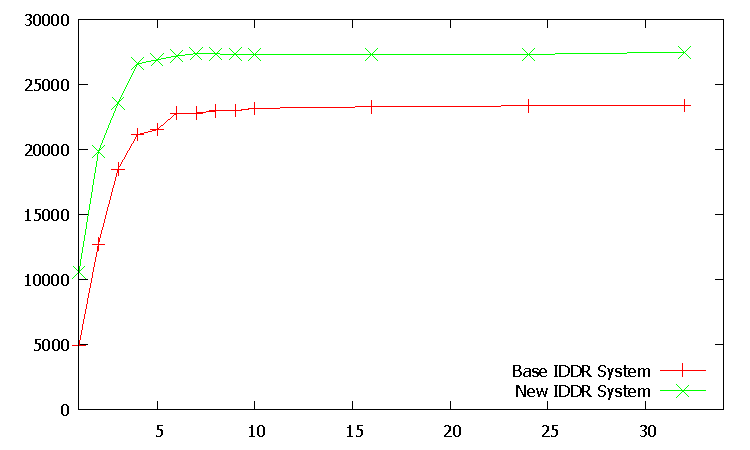
\includegraphics[scale=.7]{rndrd-ramdisk}
  \caption{Random reads}
  \label{subfig:rndrd-ramdisk}
  \end{subfigure}
  \hspace{50mm}
  \begin{subfigure}[b]{0.2\textwidth}
  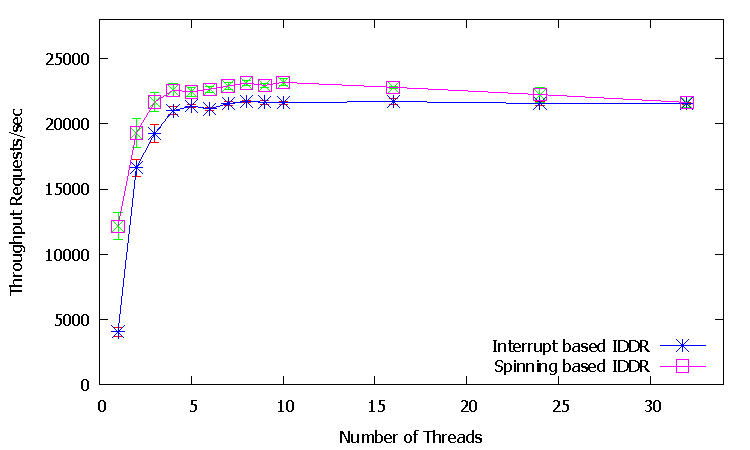
\includegraphics[scale=.7]{rndwr-ramdisk}
  \caption{Random writes}
  \label{subfig:rndwr-ramdisk}
  \end{subfigure}\\*
  \hspace{150mm}
  \begin{subfigure}[b]{0.3\textwidth}
  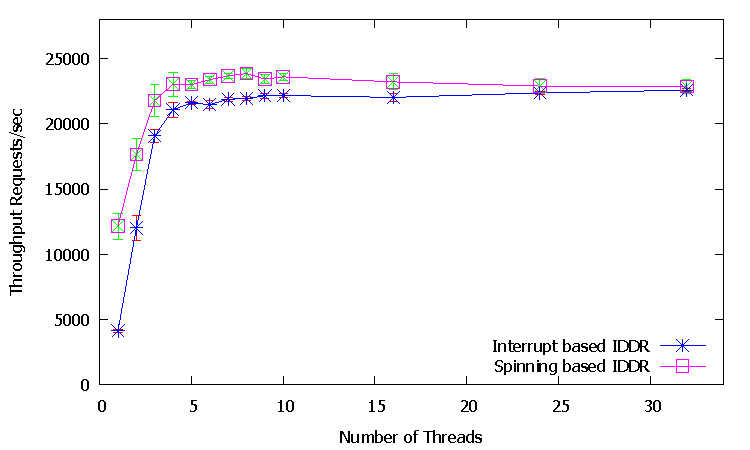
\includegraphics[scale=.7]{rndrw-ramdisk}
  \caption{Random reads writes}
  \label{subfig:rndrw-ramdisk}
  \end{subfigure}
  \caption{Random reads and writes on a Ramdisk}\label{fig:rndramdisk}
\end{figure}

\begin{figure}[!ht]
%\centering
  \begin{subfigure}[b]{0.2\textwidth}
  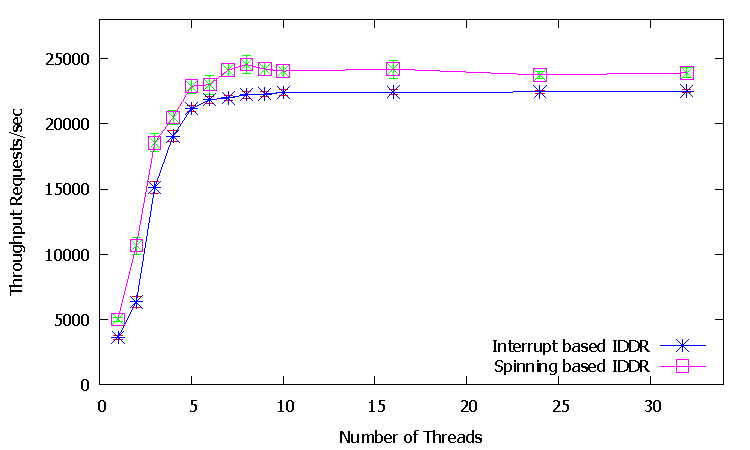
\includegraphics[scale=.7]{rndrd-loopdisk}
  \caption{Random reads}
  \label{subfig:rndrd-loopdisk}
  \end{subfigure}
  \hspace{50mm}
  \begin{subfigure}[b]{0.2\textwidth}
  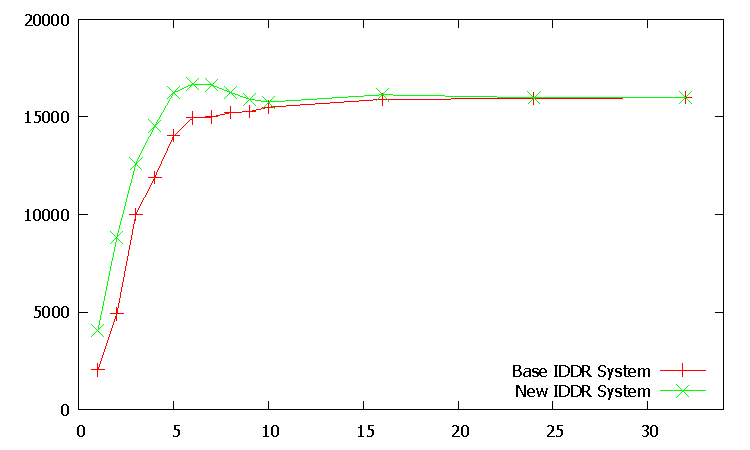
\includegraphics[scale=.7]{rndwr-loopdisk}
  \caption{Random writes}
  \label{subfig:rndwr-loopdisk}
  \end{subfigure}\\
  \begin{subfigure}[b]{0.3\textwidth}
  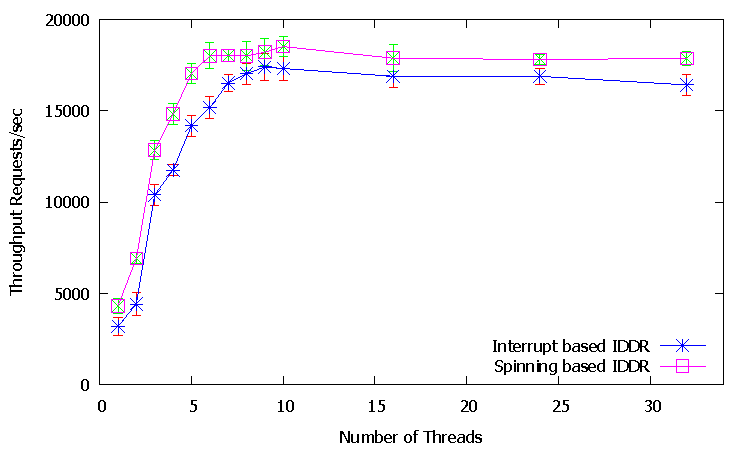
\includegraphics[scale=.7]{rndrw-loopdisk}
  \caption{Random reads writes}
  \label{subfig:rndrw-loopdisk}
  \end{subfigure}
\caption{Random reads and writes on a Loop device}\label{fig:rndloopdisk}
\end{figure}
% \pagebreak

% \paragraph{Sequential reads and writes:}
% \paragraph{Comparison :}
% Figure~\ref{fig:seqramdisk} and Figure~\ref{fig:seqloopdisk} compares the performance of the base IDDR and the new IDDR when data is read and written sequentially on a ramdisk and a loop device respectively.
% \\[3mm]
% The Figure~\ref{subfig:seqrd-ramdisk} and Figure~\ref{subfig:seqrd-loopdisk} compares the throughput, when the device is read sequentially. The graphs show that the new IDDR system performs better than the base IDDR system when the workload is not heavy. As the workload increases, the performance of the new IDDR system decreases drastically. WHY ???? ADD A REASON //TODO
% \\[3mm]
% The Figure~\ref{subfig:seqwr-ramdisk} and Figure~\ref{subfig:seqwr-loopdisk} compares the throughput of the base and new IDDR system, when the data is written on the device sequentially. The figure shows that the new IDDR systems performs better than the base IDDR system. However, the throughput improvement drops significantly as number of SysBench threads increases.
% \\[3mm]
% The Figure~\ref{subfig:seqrewr-ramdisk} and Figure~\ref{subfig:seqrewr-loopdisk} compares the throughput of the base and new IDDR system, when mixed read and writes are fired on the device sequentially. As the writing takes more time, the output is dominated by the throughput performance of the write requests. Hence, the curve is similar to the Figure~\ref{subfig:seqwr-ramdisk} and Figure~\ref{subfig:seqwr-ramdisk}. 

% \begin{figure}[!ht]
% % \centering
%   \begin{subfigure}[b]{0.2\textwidth}
%   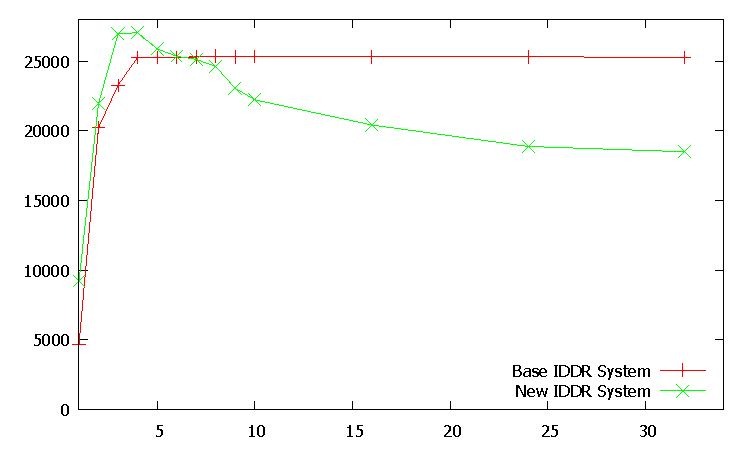
\includegraphics[scale=.7]{seqrd-ramdisk}
%   \caption{Reads}
%   \label{subfig:seqrd-ramdisk}
%   \end{subfigure}
%   \hspace{50mm}
%   \begin{subfigure}[b]{0.2\textwidth}
%   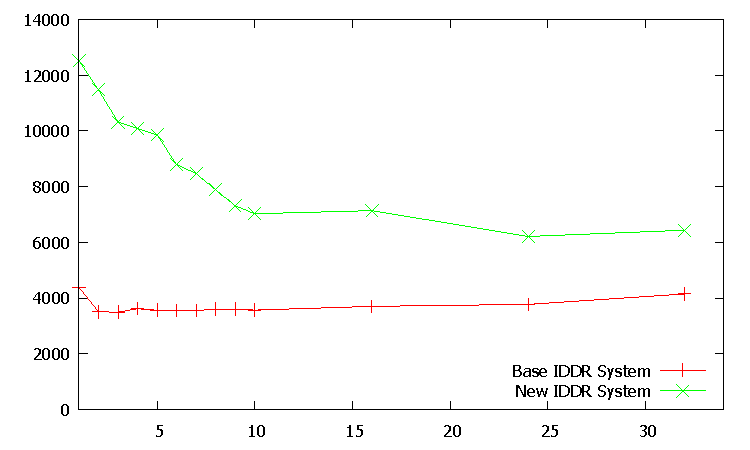
\includegraphics[scale=.7]{seqwr-ramdisk}
%   \caption{Writes}
%   \label{subfig:seqwr-ramdisk}
%   \end{subfigure}\\*
%   \hspace{150mm}
%   \begin{subfigure}[b]{0.3\textwidth}
%   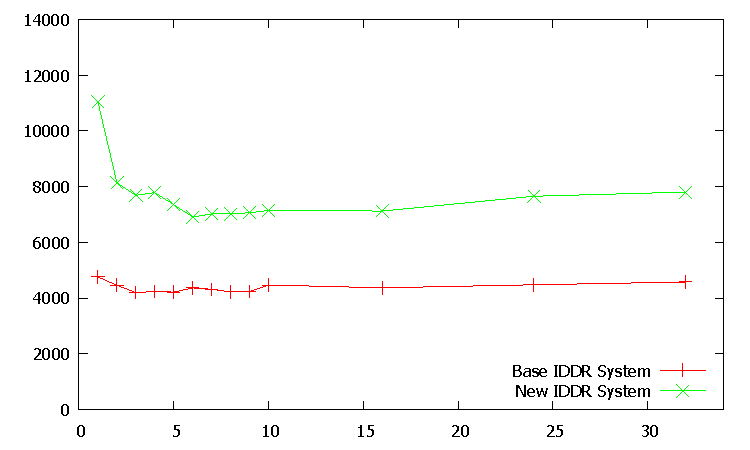
\includegraphics[scale=.7]{seqrewr-ramdisk}
%   \caption{Mix reads and writes}
%   \label{subfig:seqrewr-ramdisk}
%   \end{subfigure}
%   \caption{Sequential reads and writes on a Ramdisk}\label{fig:seqramdisk}
% \end{figure}

% \begin{figure}[!ht]
% %\centering
%   \begin{subfigure}[b]{0.2\textwidth}
%   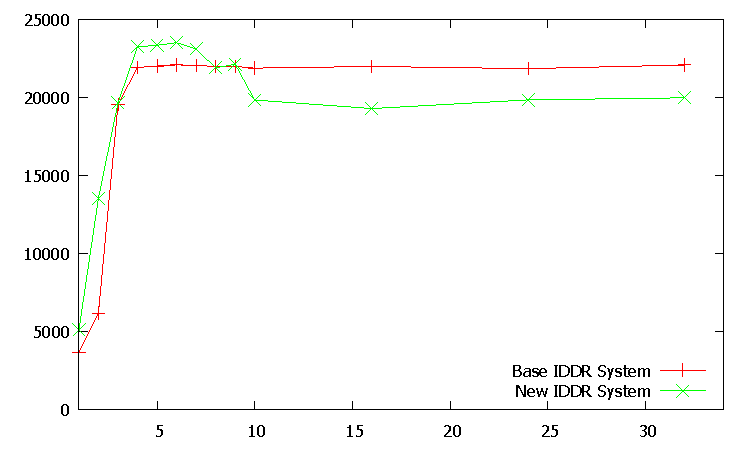
\includegraphics[scale=.7]{seqrd-loopdisk}
%   \caption{Reads}
%   \label{subfig:seqrd-loopdisk}
%   \end{subfigure}
%   \hspace{50mm}
%   \begin{subfigure}[b]{0.2\textwidth}
%   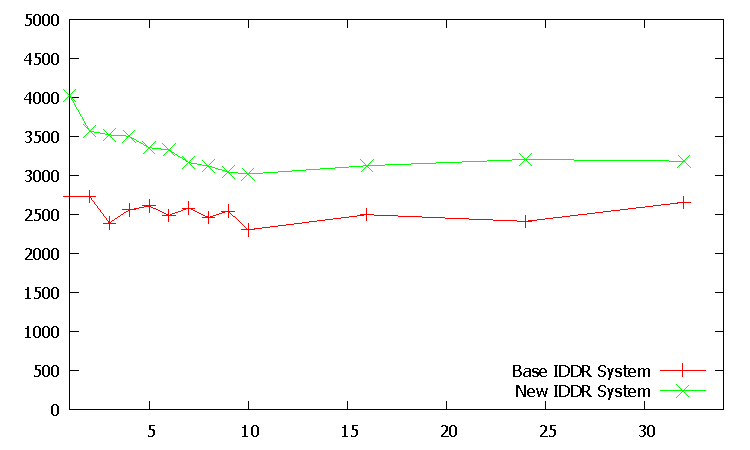
\includegraphics[scale=.7]{seqwr-loopdisk}
%   \caption{Writes}
%   \label{subfig:seqwr-loopdisk}
%   \end{subfigure}\\
%   \begin{subfigure}[b]{0.3\textwidth}
%   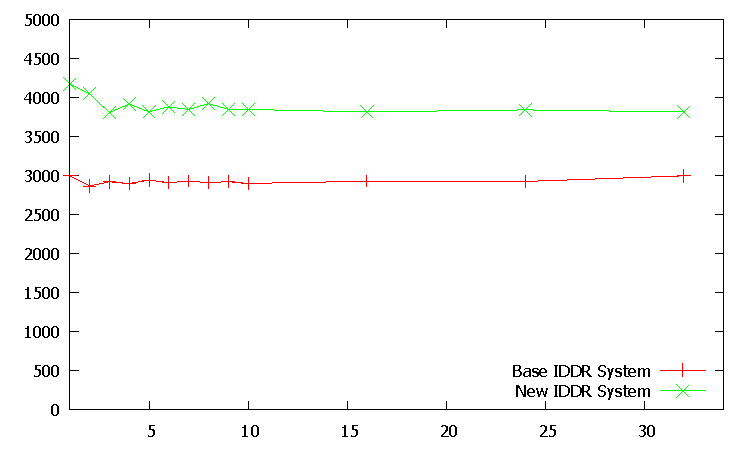
\includegraphics[scale=.7]{seqrewr-loopdisk}
%   \caption{Mix reads and writes}
%   \label{subfig:seqrewr-loopdisk}
%   \end{subfigure}
% \caption{Sequential reads and writes on a Loop device}\label{fig:seqloopdisk}
% \end{figure}


% \paragraph{Observation:}



% \begin{figure}[!ht]
% \centering
% 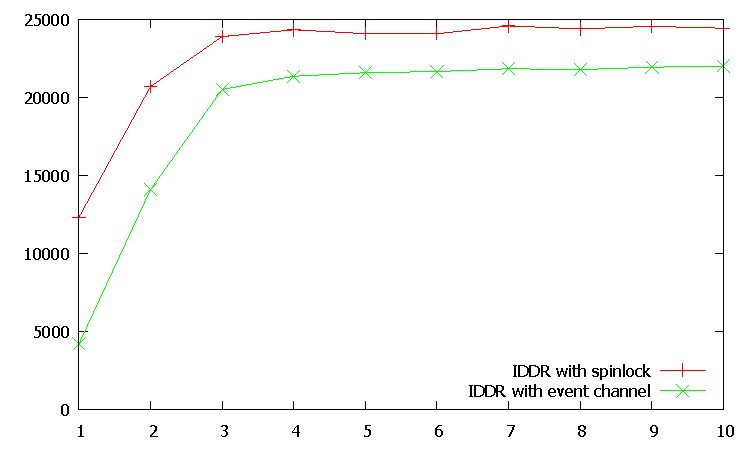
\includegraphics[scale=1]{threadvsspinram}
% \caption{The base IDDR system vs The new IDDR system (ramdisk)}
% \label{fig:threadvsspinram}
% \end{figure}
% \begin{figure}[!ht]
% \centering
% 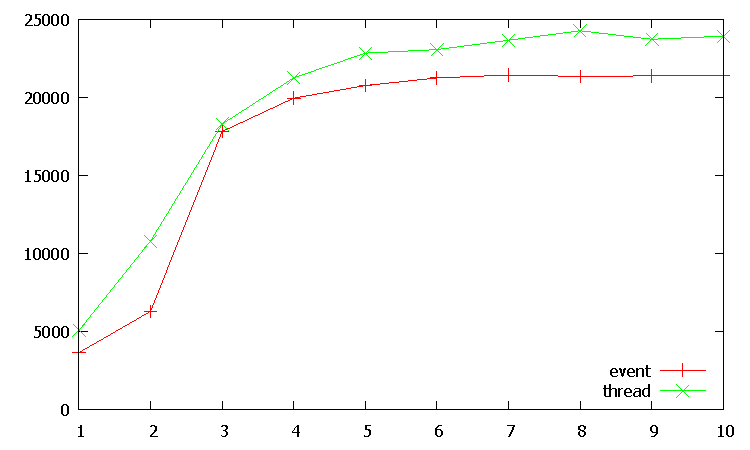
\includegraphics[scale=1]{threadvsspinloop}
% \caption{The base IDDR system vs The new IDDR system (loop device)}
% \label{fig:threadvsspinloop}
% \end{figure}


% ref
\ifbool{toShowBibliography}{\bibliography{references}}{}